\subsubsection{Iniciar Sesión}
En la figura \ref{fig:Diagrama de Secuencia - Iniciar Sesión} se muestra el diagrama de secuencia que corresponde al inicio de sesión y consta de tres partes principales: Mecánico (usuario), Sistema y Base de Datos. El objetivo es poder ingresar al sistema para poder utilizar el sistema y llevar a cabo las diversas tareas implementadas en dicho sistema. Dentro de este diagrama, existen dos opciones:
\begin{itemize}
	\item \textbf{El usuario si existe en la Base de Datos:} Hay al menos un usuario registrado con un nombre de usuario y una contraseña, posteriormente se permite el acceso al sistema con dichas credenciales.
	\item \textbf{El usuario NO existe en la Base de Datos:} No hay ningún registro de algún usuario en la base de datos, el sistema niega el acceso con esas credenciales. Cabe señalar que existe la posibilidad que el usuario ingrese de manera errónea dichas credenciales.
\end{itemize} 
\begin{figure}[!h]
	\centering
	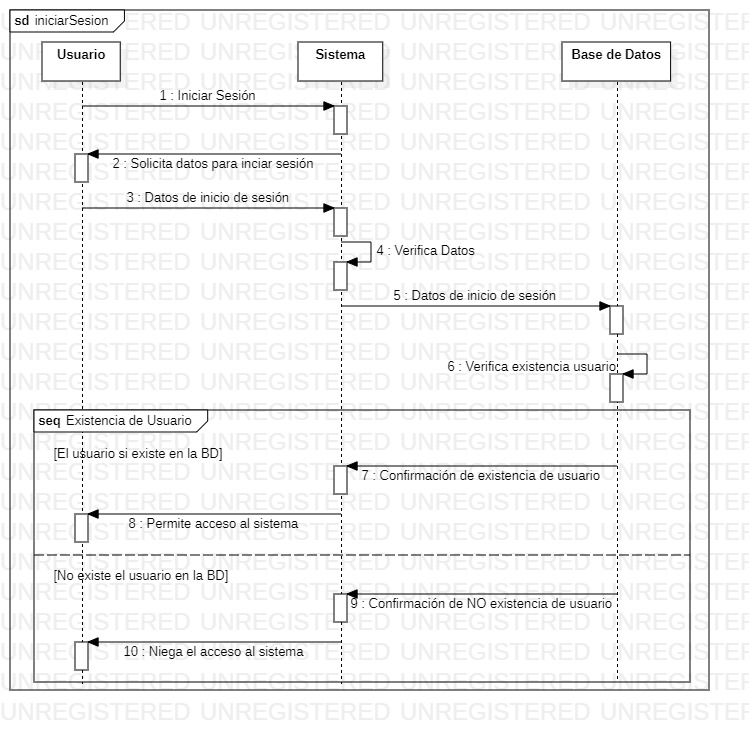
\includegraphics[width=1\textwidth]{./diseno/vprocesos/imagenes/iniciarSesion}
	\caption{Diagrama de Secuencia - Iniciar Sesión}
	\label{fig:Diagrama de Secuencia - Iniciar Sesión}
\end{figure}
\clearpage